\documentclass[]{aa} %bibnumber

%\usepackage{hyperref}
\usepackage{txfonts}
\usepackage{amsmath}
\usepackage[colorlinks,breaklinks]{hyperref}
\hypersetup{linkcolor=blue,citecolor=blue,filecolor=black,urlcolor=blue}


\usepackage{color}
\newcommand{\mr}[1]{{\textcolor[rgb]{0.60,0.10,0.6}{#1}}}
\newcommand{\mri}[1]{{\textcolor{red}{#1}}}

\def\l{\lambda}\def\L{\Lambda}

\begin{document}
\title{Redshift evolution of the SN stretch distribution}

%\subtitle{II. An example text with infinitesimal scientific value whose title
%and subtitle may also be split}

\author{N. Nicolas\inst{1}
    \and M. Rigault\inst{2}
    \and R. Graziani\inst{2}     
    \and M. Briday\inst{1}
    \and Y. Copin\inst{1}    
    \and Y. Kim\inst{1}
}

%\offprints{R. Plemmons, \email{plemmons@...}}

\institute{Université de Lyon, F-69622, Lyon, France; Université de Lyon
    1, Villeurbanne; CNRS/IN2P3, Institut de Physique des Deux Infinis, Lyon
    \and Université Clermont Auvergne, CNRS/IN2P3, Laboratoire de
    Physique de Clermont, F-63000 Clermont-Ferrand, France.
}

\date{Received 2 November 1992 / Accepted 7 January 1993}

\abstract{Type Ia supernovae (SNe Ia) allow for the construction of the Hubble
    diagram, giving us information about the Universe's expansion and its
    fondamental components, one of which is dark energy. But systematic
    uncertainties are now starting to be limiting in our ability to measure
    those parameters. In particular, the physics of SNe Ia is still mostly
    unknown, and is thought not to change in time/with the redshift.}
    {In an attempt to reduce those uncertainties, we try to find an empirical
    law describing SNe Ia's length of explosion (stretch) evolution with the
redshift.}
    {We started by getting a complete sample representing all of the stretch
        distribution that Nature can give us, before using LsSFR measurments, an
        age tracer which evolution with redshift is known, that has been shown
        to have a strong correlation with the stretch. We compare their AICc, an
    estimator of the relative quality of statistical models that includes the
number of free parameters, to determine which ones describe besto the data.}
    {Models with an evolution of the stretch with the redshift have a better
    AICc than the ones without.}
    {We find that implementing these models allows us to fit the data better
    than models without stretch evolution.}

\keywords{Cosmology -- Type Ia Supernova -- Systematic uncertainties}
\maketitle

\section{Introduction}

%\begin{figure*}
%    \centering
%    \subfigure[Method]{\label{fig:zdet}
%        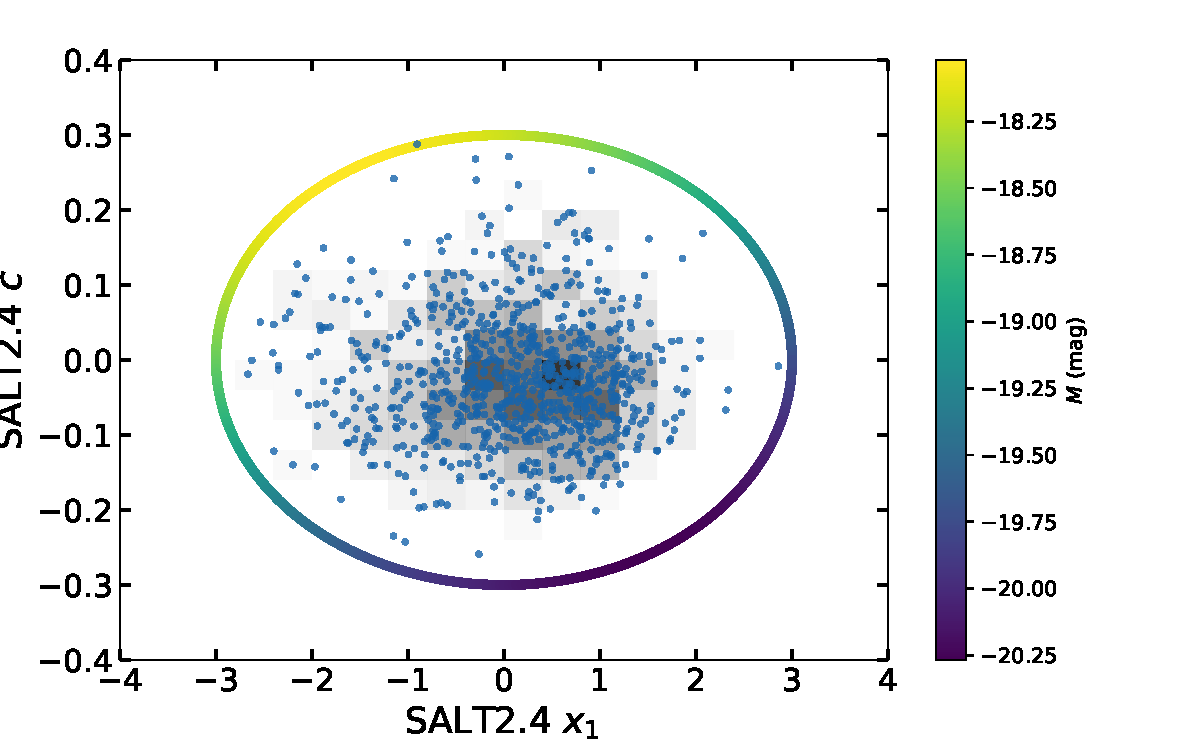
\includegraphics[width=8.5cm]{Article_figures/zmax_maglim_all.pdf}}
%    \subfigure[Result]{\label{fig:surveys_cuts}
%    \includegraphics[width=8.5cm]{A    \subfigure[Method]{\label{fig:zdet}
%rticle_figures/surveys_cuts_x.pdf}}
%    \subfigure[Method]{\label{fig:zdet}

%    \caption{(a) $z\St{max}$ determination from the magnitude limited data; (b) SDSS, %SNLS and PS1 samples cut at $z\St{max}$ as explained in
%    section \ref{sec:sam}. The data we use is in plain markers.}
%\subfigure[Method]{\label{fig:zdet}

%\end{figure*}

Type Ia supernovae (SNe Ia) are powerful cosmological distance indicators that
have enabled the discovery of the acceleration of the Universe's expansion
\citep{riess1998, permutter1999}. They remain today a key comological probe to
understand the properties of dark energy (DE) as it is the only tool able to
precisely map the recent expansion rate $z<0.5$, when DE is driving it
\citep[e.g.][]{scolnicastro2020}. They also are key to directly measure the
Hubble Constant (H$_0$) provided one can calibrate their absolute magnitude
\citep{riess2016, freedman2019}. Interestingly, the value of H$_0$ derived when
the SNeIa are anchored on Cepheids \citep[the SH0ES
project][]{riess2009,riess2016} is $\sim5~\sigma$ higher than what is predicted
by cosmic microwave background (CMB) data measured by Planck assuming the
standard $\L$CDM or when the SN luminosity is anchored at intermediate redshift
by the baryon accoustic oscillation (BAO) scale \citep{riess2019, ried2019,
planck, feeney}. While using the tip of the red giant branch technique in place
of the Cepheids seem to favor lower values of H$_0$ \citep{freedman,
recalibrationpaper} time delay measurements from strong lensing seem to also
favor high H$_0$ values \citep{wong2019}.

The H$_0$ tension has received a lot of attention as it could be a sign of new
fundamental physics. Yet, no simple solution is able to accomodate this H$_0$
tension when accounting for all other probes and the current most promising
scenario appears to be a burst of expansion at the matter-radiation decoupling
moment caused by a (fine tuned) early dark energy \citep{poulin}.

Alternatively, systematic effects affecting one or several of the aforementioned
analysis could also explain the tension. In \cite{rigault2015} we suggested that
SNe Ia from the cepheid calibrator sample differ significantly to the one from
the Hubble flow sample that enables to derive H$_0$. Indeed, Cepheid are very
young stars and the existence of Cepheids in a galaxy implies that the host is
star forming. In \citep{Rigault2015} we claimed that a more than 90\% of the
calibrator SNe Ia arise from a young-progenitor propulation while this
population only accounts for about half of the Hubble flow sample. Following
\cite{sullivan2010} and \citep{rigault2013}, we further showed that young and
old progenitor SNe Ia have a different magnitude of about 0.15 mag. This has
been confirmed for modern standardization technique
\citep[SALT2.4][]{guy2010,betoule2014} with high significance ($\sim 6\sigma$)
in \citep{rigault2018} as well as independently by \cite{roman2019} at $\sim
7\sigma$. As detailed in \citep{Rigault2015}, if the magnitude difference
between young and old SNe Ia is indeed of $0.15$ mag and if SNe Ia from the
calibrator sample is fully dominated by young SNeIa, the effect on H$_0$ of the
existance of these two SNe Ia populations is of 3.5\%. Accounting for the fact
that another environmental effect (the mass-step) is already included in the
SH0ES analysis, the net bias in the SH0ES analysis is expected closer to 3\%
\citep[see table 6 of ][]{rigault2015}. 

SHOULD BE SHORTENED A LOT: However, the importance of this astrophysical bias in
the direct measurement of H$_0$ is still highly debated. We also highlight that
it could not explain the high value of H$_0$ derived by strong lensing. First,
\cite{jones2015} did not find any environmental bias when extending the
\citep{rigault2015} study. It was more recently reported in \citep{jones2019}
that indeed local host analysis has significant influence on the SN magnitude
but much more importantly than claimed in \citep{rigault2018} and with a
connection with the progenitor physics and/or a line of sight effect that is
unclear. More importantly, \cite{riess2016} attended to mimic the cepheid sample
selection function on the Hubble flow sample by removing SNe Ia from the latter
if they classificed their host as early-type or non-star forming. They measured
that doing so has no effect on the measurement of H$_0$.

% SERIES OF PAPER
This paper is part of a series of papers where we test the validity of the two
SNe Ia population models developped in \citep{rigault2018}.Briday et al. in prep
will present how using different environmental tracer is affecting our ability
to distinguish the two populations, and Rigault et al. in prep will further
study the connection with H$_0$. Here we analyze predictions concerning the
SNe Ia redshift drifts: (1) that the distribution of the SNIa stretch, a purely
intrinsic SNIa property, is evolving as a function of redshift and (2) that this
population-drift follows the relation that \citep{rigault2018} derived assuming
that one population is “young“ with a rate proportional to the star formation
rate in the Universe and the second is "old" with a rate proportional to the
stellar mass.

The concept of the SNeIa age dichotomy arised when the SNIa rate has first been
studied. \cite{Mannucci et al. 2005; Scannapieco & Bildsten 2005; Sullivan et
al. 2006; Aubourg et al. 2008} have shown that the relative SNe Ia rate in
galaxies could only be explained if two populations existed, one young,
following the host star formation activity, and one old following the host
stellar mass (the so called “prompt and delayed“ or “A+B“ model). In
\cite{rigault2018} we used the specific star formation rate at the SN location
(Local sSFR or LsSFR) to classify which are the prompts (those with a high
LsSFR) and which are the delayed (those with low LsSFR). Since the first SNe Ia
host analysis, the SN strech has been known to be strongly correlated with the
SN host properties \citep{Hamuy1996, Hamuy2000} and it has been extensively
confirmed since \citep[e.g.][]{Neill2009,Sullivan2010; Lampeitl2010; Kelly2010;
Gupta2011,D’Andrea2011; Childress2013,Rigault2013,Pan2014}. Following the “A+B“
model and the connection between SN stretch and host properties,
\citep{Howell20XX} first discussed the potential redshift drift of the SN strech
distribution. In this paper we revisit this analysis with the most recent SNe Ia
dataset and we test the validity of the two SNIa age populations model
developped by \citep{rigault2018}.

We present in section~\ref{sec:data} the sample we are using for this analysis,
which is based on the pantheon dataset \citep{scolnic2018a}. We discuss the
importance of obtaining a "complete" sample, i.e. reprensentative of the true
underlying SNe Ia distribution, and how we build one from the Pantheon sample.
We then present in section~\ref{sec:model} our modeling of the distribution of
stretch as a function of redshift based on the relative stretch distrubtion of
young and old SNeIa. Our results are presented in section~\ref{sec:result} where
we test if the distribution of stretch does evolve as a function of redshift and
if the age-model is in good agreement with this evolution. We discuss our
results and conclude in section~\ref{sec:conclusion}.

Throughout the paper we use the Planck 2015 cosmology from the astropy library.

\section{Sample}\label{sec:sam}

We base our analysis on the latest SNe Ia compilation: the Pantheon catalog from
\cite{scolnic2018}. Using this dataset, we aim at probing the evolution of the
distribution of SNe Ia stretch in nature as a function of redshift. \mr{We thus have to }


Because the
observed magnitude of a SN Ia is correlated with its stretch and its color, in a
magnitude limited survey such as those consituing most of the Pantheon sample,
the distribution of these lightcurve parameters is not representative of the
true underlying distribution above a certain limiting redshift. The first SNe Ia
that such a survey will miss because they will be too faint are indeed the
reddest and the lowest-stretch SNe Ia. If such a selection effect is not
accounted for, we might confuse true population drift we selection function or
conversally.

The figure~\ref{fig:maglim} shows the distribution of stretch for the magnitude
limited samples of the Pantheon data, i.e. PanStarrs \citep[PS1][]{ref}, the
Sloan Digital Sky Survey \citep[SDSS][]{ref} and the SuperNovae Legacy Survey
\citep[SNLS][]{astier2006}. An ellipse in the salt2.4 $(x_1, c)$ plan with major
axis $x_1=3$ and manor axis $c=0.3$ incapsulate the full distribution \citep[see
also][for a similar contour but using a less conservative
$c=0.2$]{campbell2013}. Assuming the average SN absolute magnitude ($x_1=0$,
$c=0$) is $M=-19.36$ \citep{kessler2009,scolnic2014} we can derive the absolute magnitude of
SNeIa along this ellipse given the standardisation coefficient from
\citep{scolnic2018a}: $\alpha=0.16$ and $\beta=3.14$.

\begin{figure}
    \centering
    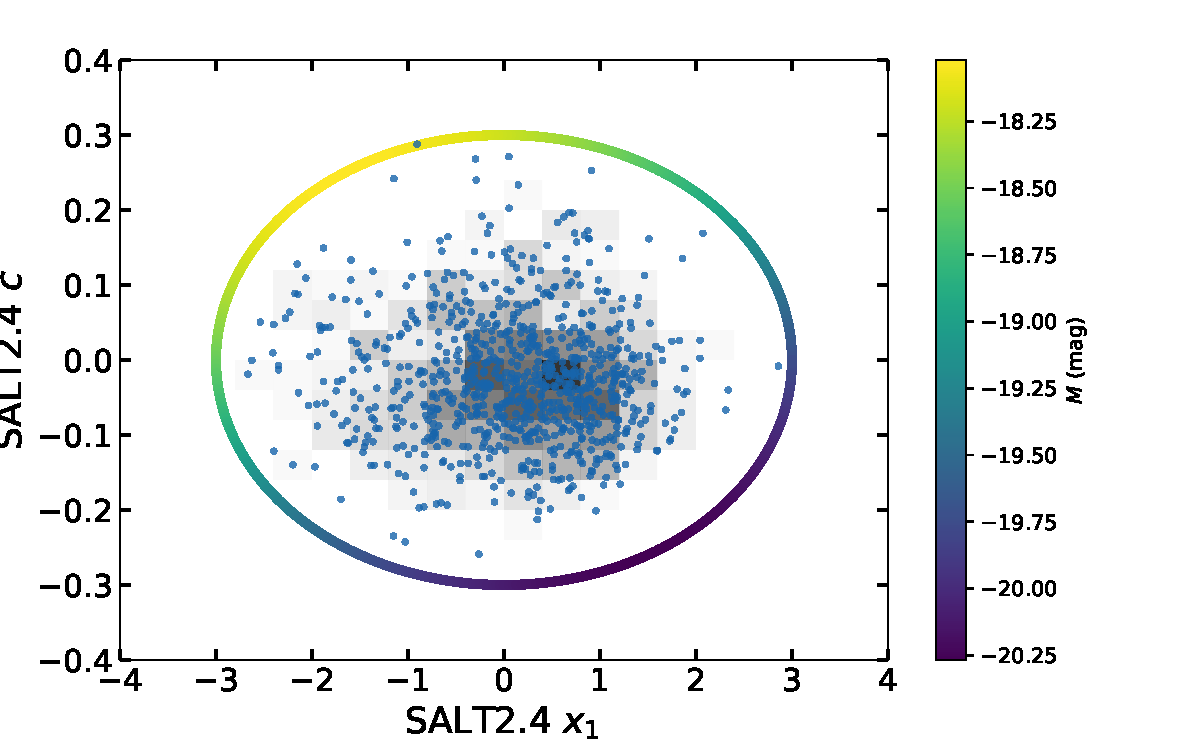
\includegraphics[width=\linewidth]{Article_figures/zmax_maglim_all.pdf}
    \caption{SALT2.4 stretch and color lightcurve parameters of SNeIa from the
        SDSS, PS1 and SNLS samples from the pantheon catalog. The individual SN
        data are shown as blue dots and a 2D histogram is shown in grey to
        highlight point density. The ellipse encapsulating all the SN data is
        displayed colored by the effective standardized absolute magnitude using
    the $\alpha$ and $\beta$ standardisation coefficents from
\citep{scolnic2018}.}
    \label{fig:maglim}
\end{figure}


The faintest SNIa is that with $x_1=-1.66$ and $c=0.25$ and has an absolute \mr{standardized} magnitude at peak \mr{in Bessel-b band} of $-18.31$ mag, which leads to limiting asbolute magnitude of
$-18.00$ if we want to be able to observe it typically a week before and 10 days after peak.  
Therefore, given the $5\sigma$ point source detection magnitude
limit of a magnitude limited survey, one can derive the maximum redshift above which the faintest SNeIa will start to be missed. 

\mr{SNLS typically acquires SNeIa in the redshift range $0.4<z<0.8$. At these redshifts the rest-frame Bessel-b band roughly corresponds to the SNLS-$i$ filter, that has a 24.8 mag $5\sigma$ depth \footnote{\href{https://www.cfht.hawaii.edu/Science/CFHTLS/cfhtlsfinalreleaseexecsummary.html}{CFHT final release website.}}. This converts to a $z_{lim}=0.60$, in perfect agreement with \citep{neill2006} and \citep{perrett2010}.
Similarly, PS1 observing SNeIa in the range $0.2<z<0.4$, their $g$-band $5\sigma$ depth is 23.1 mag \citep{rest2014}, corresponding $z_{lim}=0.30$.
The fig.~6 of \citep{scolnic2018} suggests a more conservative $z_{lim}$ of 0.27 for the PS1 catalog. In similar redshift range, SDSS has a limiting magnitude of 22.5 \citep{dilday2008,sake2008,sako2014}, which would lead to a $z_max=0.24$. However, the SDSS survey were more sensitive to limited spectroscopic ressources. \cite{kessler2009} presents that during year-1 of SDSS, SNeIa with $r-mag<20.5$ where favored for spectroscopic follow up, corresponding to the redshift cut at $0.15$. For the rest of the SDSS survey, additional spectroscopic ressources where used, such that \cite{kessler2009} and  \cite{dilday2008} of show a relative completness up to $z_{lim}=0.2$. For the rest of the analysis, we will use $z_{lim}=0.2$ as baseline magnitude.}

\mr{In Section~\ref{sec:testzmax}, we test the impact on using more conservative redshift limits ($z_{lim}=0.15$ for SDSS, $z_{lim}=0.27$ for PS and $z_{lim}=0.55$ for SNLS, following Fig.~14 of \citealt{perrett2010}).} The cuts on the raw data of those three samples are shown figure \red{fig:cuts}.

\begin{figure}
    \centering
    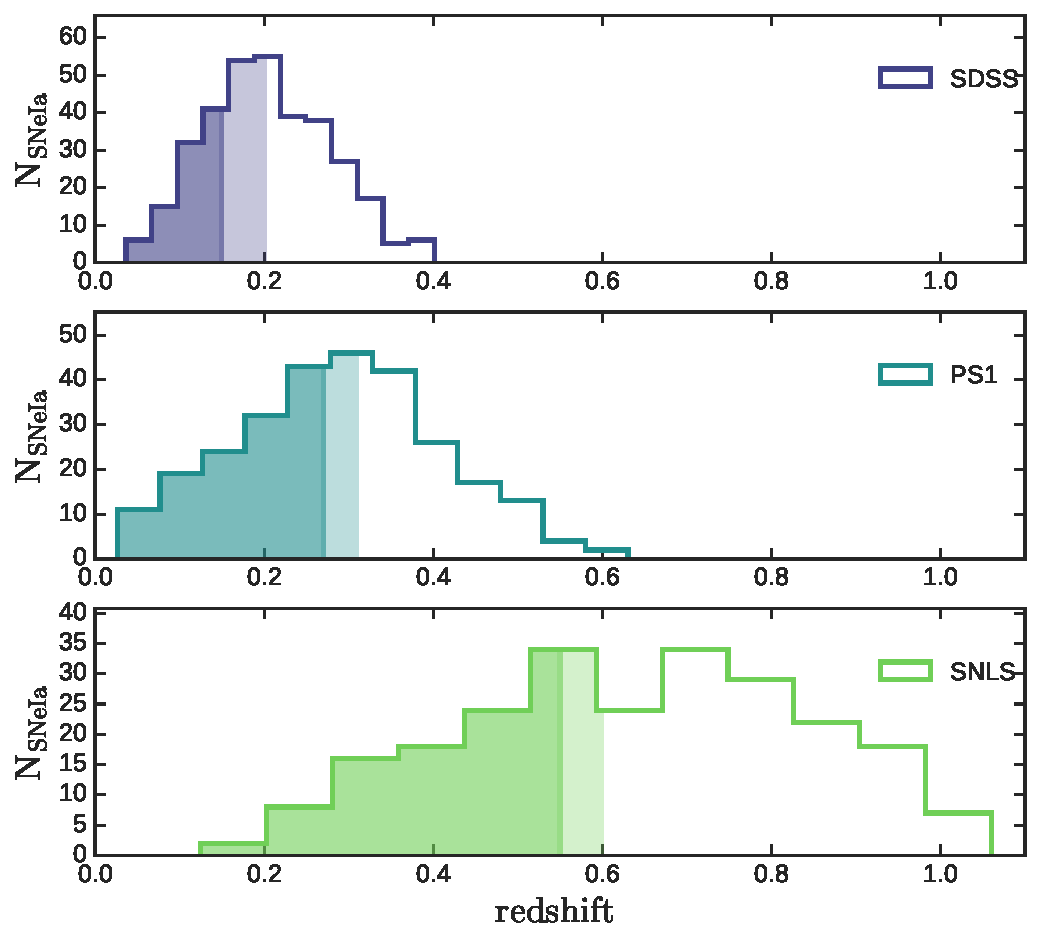
\includegraphics[width=\linewidth]{Article_figures/hist_surveys_cuts.pdf}
    \caption{Histograms of the 3 surveys on which we applied cuts to get rid of selection effects, as discussed in section \ref{sec:sam}.}
    \label{fig:cuts}
\end{figure}

In addition, we use the SNe Ia sample of from the nearby supernovae factory
\citep[SNfactory][]{aldering2004} published in \citep{rigault2018}. As the SNe
search were much deeper than the spectrophotometric follow-up, SNfactory SNe Ia
within a redshift range of $0.02<z<0.09$ should also be a random sampling of the
underlying SN population. The HST sample from
Pantheon follows the same logic and we therefore kept it entirely \citep{FIND BACK THE REF}.

Our "complete sample" is therefore made of 656 SNeIa whose composition is
detailed in table~\ref{tab:sample}.

\begin{table}
    \centering
    \caption{Origin of the SNeIa in our sample and redshift limit (if
    applicable) of each surveys.}
    \label{tab:sample}
    \begin{tabular}{l c c}
    \hline\hline\\[-0.8em]
        Survey & N$_{\mathrm{SN}}$  & z$_{lim}$ \\[0.15em]
        \hline\\[-0.8em]
        SNf & 141 & --\\[0.30em]
        SDSS & 167 & 0.20\\[0.30em]
        PS1 & 160 & 0.30 \\[0.30em]        
        SNLS & 102 & 0.60\\[0.30em]
        HST & 26 & --\\[0.30em]
        \hline
    \end{tabular}
\end{table}

%\mri{COMPARE HERE WITH LITERATURE. E.G. FIG. 6 OF SCOLNIC 2018, PS zmax AROUND0.27}

%\mri{Perrett et al. 2010 | SNLS | zmax ="z $\sim$ 0.6"}

%\mri{Dilday et al. 2008 | SDSS | sure good at z<0.12, fig. 10 suggest still okat z=0.2}

%\mri{Kessler 2009 "For the SDSS-II, the image-subtraction
%pipeline efficiency (	subtr) is complete up to a redshift of z ∼ 0.2"}

%\mri{Kesslet 2009 | "For the SDSS-II and SNLS samples, the cutoff redshifts are
%estimated to be 0.15 and 0.65, respectively."}
% ADDIND: PS cut from pantheon close to 0.27 see Fig. 6 of Scolnic 2018



\mri{CHECK LITERATURE CAN WE USE THE CfA SAMPLES ???}




\section{Method}

We used the LsSFR and stretch measurments from the SNf sample. The LsSFR has an
evolution with the redshift that is analytically known: calling $\de\z$ the
fraction of young stars and $\p\z$ the fraction of old ones, Rigault 2018 et +
find
\begin{equation}
    \frac{\delta\z}{\psi\z} \equiv \mathrm{LsSFR}\z = K\times \LF{1+z}^\varphi
\end{equation}
with $\f = 2.8$, and knowing $\de\z + \p\z = 1$:
\begin{align}
    \delta\z & = \left{K^{-1}\times \LF{1+z}^{-\f} +1\right}^{-1}\\
    \psi\z & = \LF{K\times \LF{1+z}^{+\f} + 1}\um
\end{align}

%\begin{figure*}
%    \centering
%    \subfigure[Raw data]{\label{fig:snf_data}
%        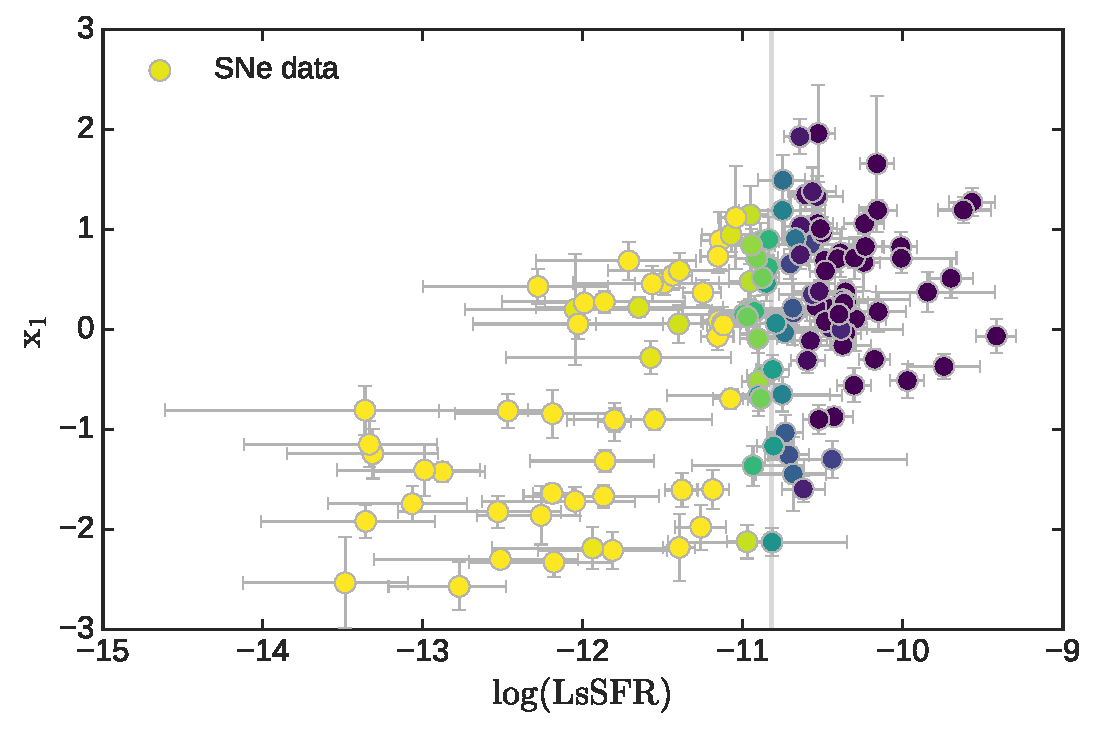
\includegraphics[width=8.5cm]{Article_figures/BiGaussian_onlydata.pdf}}
%    \subfigure[First implemented model]{\label{fig:3G2M2SSNF}
%        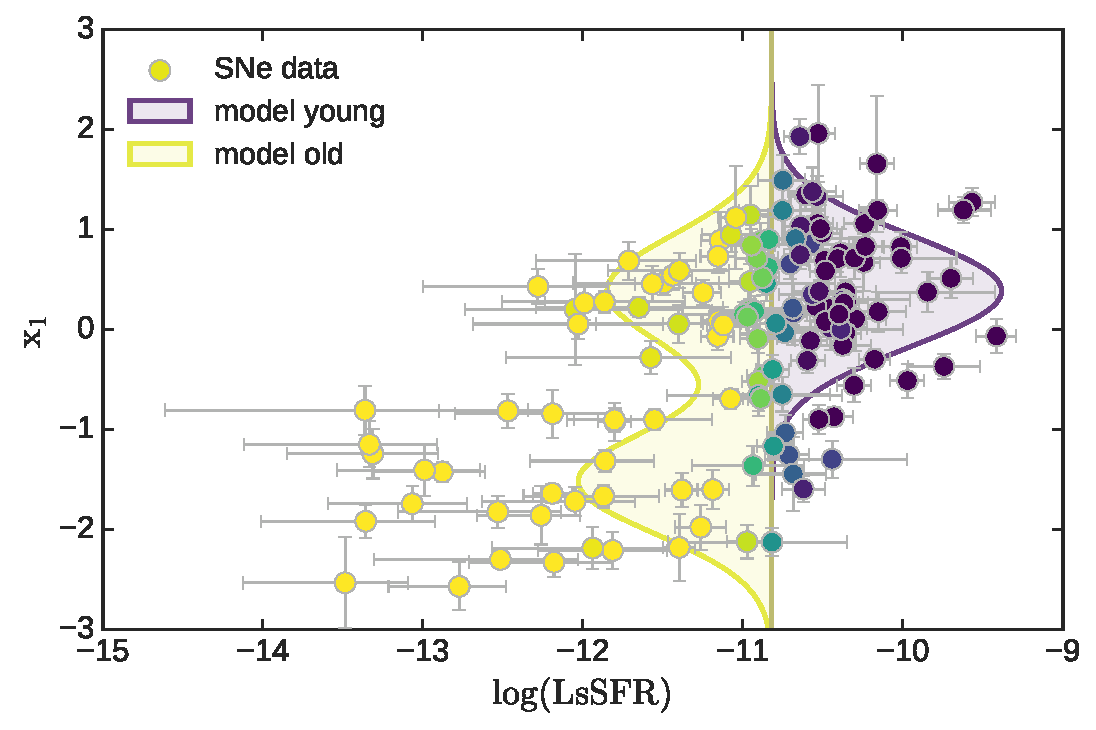
\includegraphics[width=8.5cm]{Article_figures/BiGaussian.pdf}}
%    \caption{Stretch des supernovae étudiées par la collaboration SNF en
%    fonction de log(LsSFR). La couleur représente la probabilité pour une
%supernova d'être issue d'un jeune progéniteur.}
%    \label{fig:mod_first}
%\end{figure*}

The goal is to find how the stretch depends on the LsSFR, distinguishing old and
young SNe which fractions evolve with the redshift, in order to have an
analytical law for the mean redshift evolution of the stretch. The measured data
on which we based our first model is plotted in figure \ref{fig:mod_first};
based of the shape of the $x_1$ vs LsSFR cloud, we implemented the following
model:
\begin{itemize}
    \item \textbf{young}: a gaussian of mean $\m_1$ and standard deviation
        $\s_1$, namely $\Nc_1 \equiv \Nc \LF{\m_1,\s_1}$;
    \item \textbf{old}: a linear combination between $\Nc_1$ and another
        gaussian $\Nc_2 \equiv \Nc \LF{\m_2,\s_2}$
\end{itemize}
As such, the probability to observe a young SNe Ia labeled "i" with a stretch
$x_1^i$ and error $\d x_1^i$ is
\begin{equation}
    p \LF{x_1^i, \d x_1{}^i|\m_1,\s_1} = \Nc \LF{\m_1, \Sq{\s_1{}^2 + \d
    x_1^i{}^2}}(x_1^i)
\end{equation}
and for an old one:
\begin{align}
    p(x_1^i, \d x_1^i | \m_{1,2}, \s_{1,2}, a) = a & \times \Nc \LF{\m_1,
    \sqrt{\s_1{}^2 + \d x_1^i{}^{2}}} (x_1^i) \ + \\ (1-a) & \times \Nc
    \LF{\m_2, \sqrt{ \s_2{}^2 + \d x_1^i{}^{2}}} (x_1^i), \nonumber 
\end{align}

\noindent where $a$ is the relative amplitude between the two gaussians.
Finally, the normalized stretch distribution at a given $z$ $\D\LF{x_1|z}$ is
the weigthed sum of both young and old stretch distributions given their
relative fraction $\de\z$:
\begin{equation}
    \D\LF{x_1|z} = \de\z\times\Nc_1 +
    \LF{1-\de\z} \times \LF{a\Nc_1 + (1-a)\Nc_2}
\end{equation}

We fitted it on SNf data, giving the results table \ref{tab:val}, with a graphical representation shown figure \ref{fig:snf_model}. For clarity
with the next models, we named it 3G2M2S$\St{SNf}$ for it has a total of 3
gaussians but with only 2 means and 2 standard deviations, and has been fitted
on SNf data only. 

\begin{figure}
    \centering
    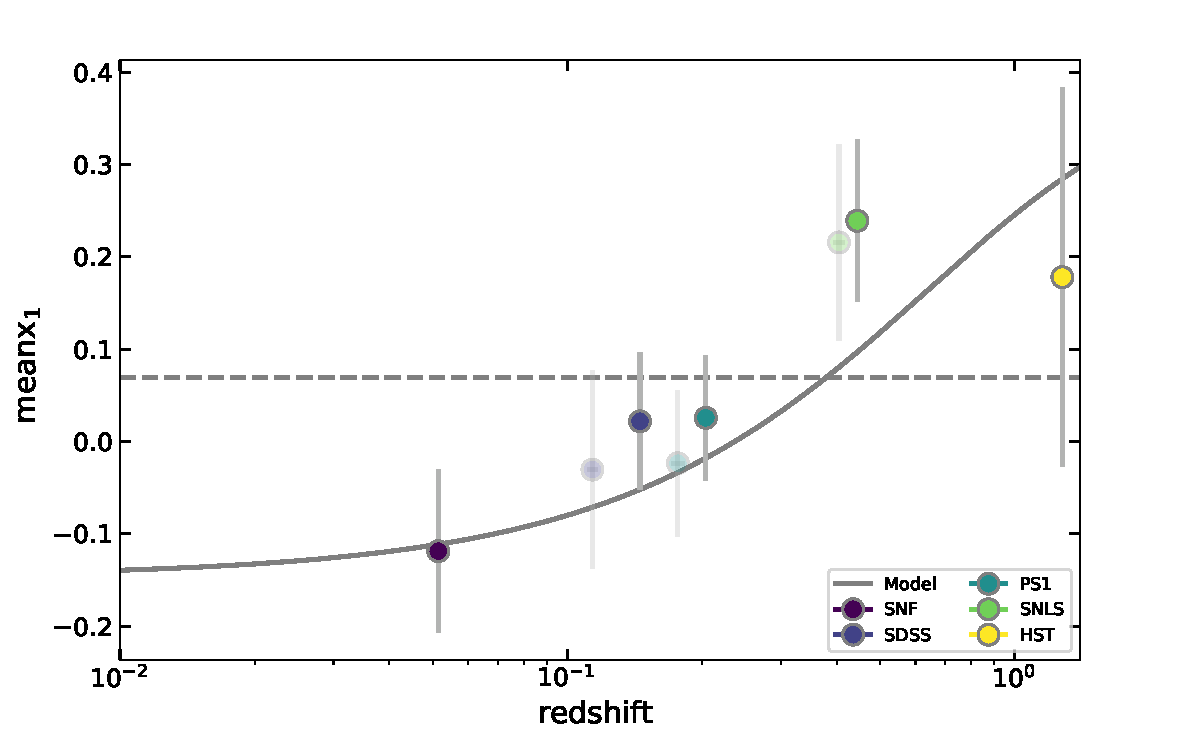
\includegraphics[width=\linewidth]{Article_figures/stretchevol_model_maglim-cuts.pdf}
    \caption{Result of the model fitted on SNF data and mean of stretch and redshift of the other surveys used for this analysis. Conservative data is shown in transparent markers.}
    \label{fig:snf_model}
\end{figure}

We implemented and compared 10 models in total, 4 of which have an
evolution with the redshift from $\de\z$, and 6 don't ($\de\z = f =
\mathrm{cst}$). The ones with and evolution are:
\begin{itemize}
    \item 3G2M2S, the one we described (but fitted on all the data);
    \item 3G2M1S, where this time $\s_1 \equiv \s_2$;
    \item 2G2M2S, model taken from HOWELL 2009 where we added $\de\z$;
    \item 3G3M3S, with three independent gaussians.
\end{itemize}
The ones without a stretch evolution are the same ones but with an "F" implying
we set $\de\z = f = \mathrm{cst}$, and two others:
\begin{itemize}
    \item 1G1M1S, where there is no distinction between old and young SNe;
    \item 1G1M2S, taken from KESLLER 2017 and used in recent cosmological
        analysis SCOLNIC 2018. It's an asymetric model where
\end{itemize}
\begin{align}
 p(x_1^i, \d x_1^i | \m, \s_-, \s_+) = 
    \begin{cases}
        \mathcal{N} \LF{\m, \sqrt{\s_-{}^2 + \d x_1^i{}^{2}}} (x_1^i) & \text{if
        } x_1^i\geq \m\\
        \mathcal{N} \LF{\m, \sqrt{\s_+{}^2 + \d x_1^i{}^{2}}} (x_1^i), &
        \text{else}
    \end{cases}
\end{align} 

The fitted parameters are showed table \ref{tab:val}.

\begin{table*}[htbp!]
    \centering
    \caption{Valeurs des paramètres pour différents modèles. En rouge les
    données aberrantes.}
    \label{tab:val}
    \begin{tabular}{c c c c c c c}\hline\hline

        Model & $a$ & $f$ & $\m_1$ & $\s_1$ & $\m_2$ &
        $\s_2$ \\\hline

        3G2M2S$_{\mathrm{SNf}}$ & $0.48 \pm 0.07$ & none & $0.39 \pm 0.07$ &
        $0.56 \pm 0.05$ & $-1.5 \pm 0.1$ & $0.52 \pm 0.09$ \\

        3G2M2S & $0.48 \pm 0.17$ & none & $0.36 \pm 0.08$ & $0.61 \pm 0.05$ &
        $-1.3 \pm 0.2$ & $0.60 \pm 0.12$ \\

        3G2M2SF & \textcolor{red}{$0.1 \pm 0.6$} & \textcolor{red}{$0.2 \pm
        0.6$} & $-0.9 \pm 0.7$ & $0.7 \pm 0.3$ & $0.5 \pm 0.2$ & $0.6 \pm 0.1$
        \\

        3G2M1S & $0.47 \pm 0.07$ & none & $0.35 \pm 0.04$ & $0.61 \pm 0.03$ &
        $-1.25 \pm 0.10$ & $\s_1$ \\

        3G2M1SF & \textcolor{red}{$0.2 \pm 0.9$} & $0.7 \pm 0.3$ & $0.36 \pm
        0.04$ & $0.60 \pm 0.03$ & $-1.23 \pm 0.10$ & $\s_1$ \\

        2G2M2S & none & none & $0.49 \pm 0.04$ & $0.54 \pm 0.03$ & $-0.72 \pm
        0.08$ & $0.83 \pm 0.07$ \\
        
        2G2M2SF & none & $0.3 \pm 0.2$ & $-0.9 \pm 0.6$ & $0.7 \pm 0.2$ & $0.5
        \pm 0.2$ & $0.56 \pm 0.09$ \\\hline

    \end{tabular} \bigbreak

\begin{tabular}{c c c}\hline\hline

    Model & $\m$ & $\s$ \\\hline

    1G1M1S & $0.01 \pm 0.04$ & $0.90 \pm 0.03$ \\\hline

\end{tabular} \bigbreak

\begin{tabular}{c c c c c}\hline\hline

    Model & $\m$ & $\s_-$ & $\s_+$ \\\hline

    1G1M2S & $0.16617 \pm 0.00004$ & $1.07 \pm 0.04$ & $0.69 \pm 0.03$ \\\hline

\end{tabular} \bigbreak

\begin{tabular}{c c c c c c c c c}\hline\hline

    Model & $a$ & $f$ & $\m_1$ & $\s_1$ & $\m_2$ & $\s_2$ &
    $m_3$ & $\s_3$ \\\hline

    3G3M3S & $0.14 \pm 0.08$ & none & $0.51 \pm 0.06$ & $0.54 \pm 0.04$ & $-1.9
    \pm 0.2$ & $0.29 \pm 0.11$ & $-0.55 \pm 0.12$ & $0.67 \pm 0.15$ \\
    
    3G3M3SF & $0.2 \pm 0.2 $ & $0.10 \pm 0.04 $ & $-1.7 \pm 0.2$ & $0.4 \pm 0.1$
            & $0.9 \pm 0.1$ & $0.3 \pm 0.2$ & $0.0 \pm 0.2$ & $0.7 \pm 0.1$
            \\\hline

\end{tabular} \bigbreak

\end{table*}

To test the coherence of this model, we also fitted it using all the data from the surveys indistinctly. These results are shown figures \ref{fig:model_all} and \ref{fig:model_all_cons}


\begin{figure}
    \centering
    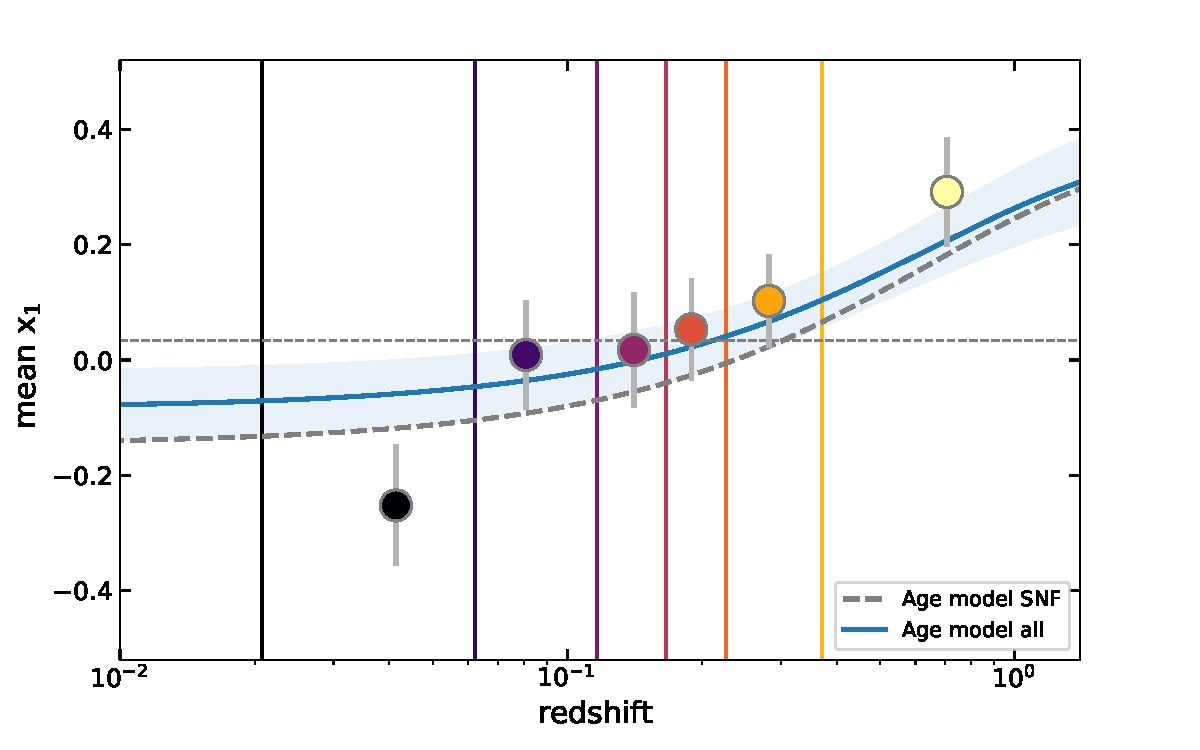
\includegraphics[width=\linewidth]{Article_figures/stretchevol_all_vs_snf_maglim_sup.pdf}
    \caption{Result of the model fitted on all surveys data cut at the non-conservative $z_{\mathrm{max}}$. We chose the bins to compute the means of stretch and redshift by making them equal in number of SNe Ia.}
    \label{fig:model_all}
\end{figure}

\begin{figure}
    \centering
    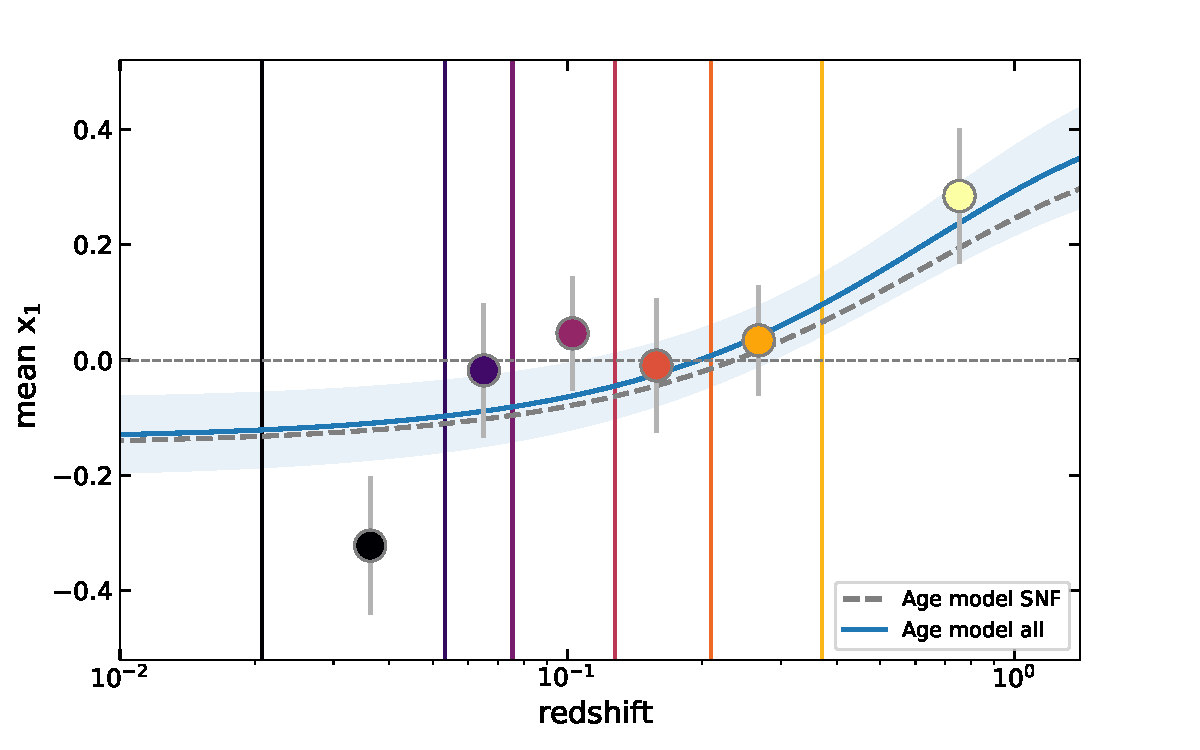
\includegraphics[width=\linewidth]{Article_figures/stretchevol_all_vs_snf_maglim_inf.pdf}
    \caption{Result of the model fitted on all surveys data cut at the conservative $z_{\mathrm{max}}$. We chose the bins to compute the means of stretch and redshift by making them equal in number of SNe Ia.}
    \label{fig:model_all}
\end{figure}

\section{Results}
To compare all these models, we use the Akaike Information Criterion corrected
for sample size (BURNHAM 2002), that penalises the increase of free parameters
in order to discourage overfitting:
\begin{equation}
    \mathrm{AICc} = \mathrm{AIC} + \LR{2k\LF{k+1}}{n - k - 1}
\end{equation}
with $\mathrm{AIC} = 2k - 2\ln\LF{\mathcal{L}}$, where $k$ is the number of free
parameters and $\Lc$ the likelihood. The probability for a model to be as
representative as the "best" one is given by:
\begin{equation}
    p(\mathrm{other} > \mathrm{best}) = \exp\LF{\D\mathrm{AICc}/2}
\end{equation}
The results are showed table \ref{tab:comp}. We find that every model lacking an
evolution of the stretch with the redshift is systematically worse than those
that implement it.

\begin{table*}[htbp!]
    \centering
    \caption{Comparaison des modèles. NR représente les modèles implémentés
             durant ce stage. (F) indique les modèles pour lesquels il n'y a pas
             d'évolution de la fraction de SNe~Ia jeunes et vieilles en fonction
             du redshift.}
    \label{tab:comp}
    \begin{tabular}{c c c c c c c}\hline\hline

        Name & Description & Free param &
        $\ln\mathcal{L}$ & $AICc$ & $\D AICc$ & Proba \\\hline

        3G2M1S & NR 1S & 4 & 1815 & 1823 & 0.0 & $1.0$ \\

        3G2M2S & NR 2S & 5 & 1815  & 1825 & -2.0 & $3.6\times10^{-1}$ \\

        2G2M2S & Howell & 4 & 1818  & 1826 & -3.4 & $1.8\times10^{-1}$ \\

        3G3M3S & NR 3S & 7 & 1812  & 1826 & -3.6 & $1.6\times10^{-1}$ \\

        3G3M3SF & NR 3S (F) & 8 & 1813 & 1829 & -6.3  & $4.3\times10^{-2}$
        \\

        2G2M2SF & Howell (F) & 5 & 1823  & 1833 & -9.9 & $7.0\times10^{-3}$
        \\

        3G2M1SF & NR 1S (F) & 5 & 1823  & 1833 & -10.4 & $5.5\times10^{-3}$
        \\

        3G2M2SF & NR 2S (F) & 6 & 1823  & 1835 & -12.0 & $2.5\times10^{-3}$
        \\

        1G1M2S & Kessler (F) & 3 & 1837  & 1843 & -20.2 & $4.1\times10^{-5}$
        \\

        1G1M1S & 1 gauss. (F) & 2 & 1872 & 1876 & -53.5 &
        $2.4\times10^{-12}$\\\hline

    \end{tabular}
\end{table*}

\section{Conclusion}
Stretch evolution with the redshift is a thing. Need to see if it has an impact
on the cosmology though.


\begin{acknowledgements}
    This project has received funding from the European Research Council (ERC) under the European Union's Horizon 2020 research and innovation programme (grant agreement n 759194 - USNAC). Support has been provided by the Institut Universitaire de France, the CNES, and the region Auvergne-Rhone-Alpes.
\end{acknowledgements}

\bibliographystyle{aa} % style aa.bst
\begin{thebibliography}{} 
% A
\bibitem[Abbott et al.(2018)]{abbott2018} Abbott, T.~M.~C., Abdalla, F.~B., Alarcon, A., et al.\ 2018, \prd, 98, 043526

\bibitem[Ata et al.(2017)]{ata2017} Ata, M., Kitaura, F.-S., Chuang, C.-H., et al.\ 2017, \mnras, 467, 3993


% B
% C
\bibitem[Chabanier et al.(2019)]{chabanier2019} Chabanier, S., Millea, M., \& Palanque-Delabrouille, N.\ 2019, \mnras, 489, 2247
\bibitem[Coles, \& Jones(1991)]{coles1991} Coles, P., \& Jones, B.\ 1991, \mnras, 248, 1


% D
% E
% F
\bibitem[Freedman et al.(2019)]{freedman2019} Freedman, W.~L., Madore, B.~F., Hatt, D., et al.\ 2019, \apj, 882, 34

% G

%\bibitem[Graziani et al.(2019)]{graziani2019} Graziani, R., Courtois, H.~M., Lavaux, G., et al.\ 2019, \mnras, 488, 5438

% H
% I 
% J
\bibitem[Jones et al.(2018)]{jones2018} Jones, D.~O., Riess, A.~G., Scolnic, D.~M., et al.\ 2018, \apj, 867, 108

% K

\bibitem[Knox, \& Millea(2019)]{knox2019} Knox, L., \& Millea, M.\ 2019, arXiv e-prints, arXiv:1908.03663

% L

% M
% N
% O
% P
\bibitem[Poulin et al.(2019)]{poulin2019} Poulin, V., Smith, T.~L., Karwal, T., et al.\ 2019, \prl, 122, 221301

\bibitem[Planck Collaboration et al.(2018)]{planck2018} Planck Collaboration, Aghanim, N., Akrami, Y., et al.\ 2018, arXiv e-prints, arXiv:1807.06209

% Q
% R
\bibitem[Reid et al.(2019)]{reid2019} Reid, M.~J., Pesce, D.~W., \& Riess, A.~G.\ 2019, arXiv e-prints, arXiv:1908.05625


\bibitem[Riess et al.(2016)]{riess2016} Riess, A.~G., Macri, L.~M., Hoffmann, S.~L., et al.\ 2016, \apj, 826, 56

\bibitem[Riess et al.(2019)]{riess2019} Riess, A.~G., Casertano, S., Yuan, W., et al.\ 2019, \apj, 876, 85



\bibitem[{Rigault {et~al.}(2013)}]{rigault2013}
Rigault, M., Copin, Y., Aldering, G., {et~al.} 2013, \aap, 560, A66

\bibitem[Rigault et al.(2015)]{rigault2015} Rigault, M., Aldering, G., Kowalski, M., et al.\ 2015, \apj, 802, 20


\bibitem[Rigault et al.(2018)]{rigault2018} Rigault, M.,
  Brinnel, V., Aldering, G., et al.\ 2018, arXiv:1806.03849
% S
\bibitem[Scolnic et al.(2018)]{scolnic2018} Scolnic, D.~M., Jones, D.~O., Rest, A., et al.\ 2018, \apj, 859, 101

% T
% U 
% V
% W
\bibitem[Wong et al.(2019)]{wong2019} Wong, K.~C., Suyu, S.~H., Chen, G.~C.-F., et al.\ 2019, arXiv e-prints, arXiv:1907.04869

% X
% Y
 Z
\end{thebibliography}


\end{document}
